\begin{figure}
    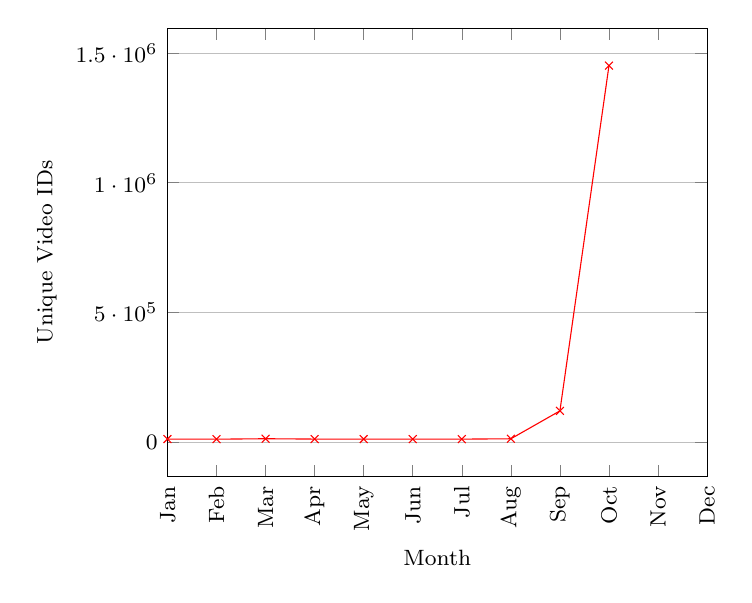
\begin{tikzpicture}
        \begin{axis}[
            xmin = 1,
            xmax = 12,
            xlabel = Month,
            ylabel = Unique Video IDs,
            scaled y ticks = false,
            ymajorgrids = true,
            x tick label style = {rotate=90, anchor=east},
            xtick = {1, ..., 12},
            xticklabels = {Jan, Feb, Mar, Apr, May, Jun, Jul, Aug, Sep, Oct, Nov, Dec},
            font = \footnotesize
            ]
            \addplot[color=red, mark=x] coordinates {
                (1, 11603)
                (2, 11194)
                (3, 12907)
                (4, 11581)
                (5, 11572)
                (6, 11609)
                (7, 11410)
                (8, 12716)
                (9, 120304)
                (10, 1451846)
            };
         %   \addplot[color=blue, mark=*] coordinates {
         %       (1, 11603)
         %       (2, 11402)
         %       (3, 12905)
         %       (4, 11581)
         %       (5, 11527)
         %       (6, 11640)
         %       (7, 11206)
         %       (8, 12709)
         %       (9, 110822)
         %       (10, 1280155)
         %   };
        \end{axis}
    \end{tikzpicture}
    \caption{Unique video IDs for 2015, by month}
    \label{2015-video-ids}
\end{figure}
